% Version 3 December 2023
% See section 11 of the User Manual for version history
%
%%%%%%%%%%%%%%%%%%%%%%%%%%%%%%%%%%%%%%%%%%%%%%%%%%%%%%%%%%%%%%%%%%%%%%
%%                                                                 %%
%% Please do not use \input{...} to include other tex files.       %%
%% Submit your LaTeX manuscript as one .tex document.              %%
%%                                                                 %%
%% All additional figures and files should be attached             %%
%% separately and not embedded in the \TeX\ document itself.       %%
%%                                                                 %%
%%%%%%%%%%%%%%%%%%%%%%%%%%%%%%%%%%%%%%%%%%%%%%%%%%%%%%%%%%%%%%%%%%%%%

%%\documentclass[referee,sn-basic]{sn-jnl}% referee option is meant for double line spacing

%%=======================================================%%
%% to print line numbers in the margin use lineno option %%
%%=======================================================%%

%%\documentclass[lineno,sn-basic]{sn-jnl}% Basic Springer Nature Reference Style/Chemistry Reference Style

%%======================================================%%
%% to compile with pdflatex/xelatex use pdflatex option %%
%%======================================================%%

%%\documentclass[pdflatex,sn-basic]{sn-jnl}% Basic Springer Nature Reference Style/Chemistry Reference Style

%%Note: the following reference styles support Namedate and Numbered referencing. By default the style follows the most common style. To switch between the options you can add or remove “Numbered” in the optional parenthesis.\\

%%The option is available for: sn-basic.bst, sn-vancouver.bst, sn-chicago.bst%

%%\documentclass[pdflatex,sn-nature]{sn-jnl}% Style for submissions to Nature Portfolio journals
%%\documentclass[pdflatex,sn-basic]{sn-jnl}% Basic Springer Nature Reference Style/Chemistry Reference Style
\documentclass[pdflatex, sn-mathphys-num, lineno]{sn-jnl}% Math and Physical Sciences Numbered Reference Style
%%\documentclass[pdflatex,sn-mathphys-ay]{sn-jnl}% Math and Physical Sciences Author Year Reference Style
%%\documentclass[pdflatex,sn-aps]{sn-jnl}% American Physical Society (APS) Reference Style
%%\documentclass[pdflatex,sn-vancouver,Numbered]{sn-jnl}% Vancouver Reference Style
%%\documentclass[pdflatex,sn-apa]{sn-jnl}% APA Reference Style
%%\documentclass[pdflatex,sn-chicago]{sn-jnl}% Chicago-based Humanities Reference Style

%%%% Standard Packages
%% additional latex packages if required can be included here>
\usepackage{graphicx}%
\usepackage{multirow}%
\usepackage{amsmath,amssymb,amsfonts}%
\usepackage{amsthm}%
\usepackage{mathrsfs}%
\usepackage[title]{appendix}%
\usepackage{xcolor}%
\usepackage{textcomp}%
\usepackage{manyfoot}%
\usepackage{booktabs}%
\usepackage{algorithm}%
\usepackage{algorithmicx}%
\usepackage{algpseudocode}%
\usepackage{listings}%

\usepackage{xspace}
\usepackage{standalone}

%% my package start

% for collabration and will remove before submit
\newcommand{\yy}[1]{\textcolor{cyan}{\textbf{[Yangyang: #1]}}}
\newcommand{\rd}[1]{\textcolor{green}{\textbf{[Dr.Yang: #1]}}}
\newcommand{\ty}[1]{\textcolor{orange}{\textbf{[Tingyou: #1]}}}
\newcommand{\qx}[1]{\textcolor{purple}{\textbf{[Qingxiang: #1]}}}

% for collabration and will remove before submit

\usepackage[detect-all=true]{siunitx}
\sisetup{
    scientific-notation=false,
    round-mode = places,
    round-precision = 0
}


\usepackage[acronym, automake, style=index, shortcuts]{glossaries-extra}
\setabbreviationstyle[acronym]{long-short}
% define glossaries
\makeglossaries

\newacronym{blat}{BLAT}{BLAST-like alignment tool}
\newacronym{llm}{LLM}{Large Language Model}
\newacronym{hmm}{HMM}{Hidden Markov Model}
\newacronym{gpu}{GPU}{Graphics Processing Unit}
\newacronym{hpc}{HPC}{High Performance Computing}
\newacronym{bert}{BERT}{Bidirectional Encoder Representations from Transformers}
\newacronym{gpt}{GPT}{Generative Pre-trained Transformer}

\newacronym{ide}{IDE}{Integrated Development Environment}
\newacronym{cd}{CD}{Continuous Development}
\newacronym{ucsc}{UCSC}{UCSC Genome Browser}
\newacronym{glm}{GLM}{Genomic Language Model}
\newacronym{lcglm}{LCGLM}{long-context genomic language model}
\newacronym{snp}{SNP}{Single Nucleotide Polymorphism}
\newacronym{fm}{FM}{Foundational Model}
\newacronym{nlp}{NLP}{Natural Language Processing}

\newacronym{mlp}{MLP}{multilayer perceptron}
\newacronym{drs}{DRS}{direct RNA sequencing}
\newacronym{ont}{ONT}{Oxford Nanopore Technologies}
\newacronym{pb}{PacBio}{Pacific Biosciences}

\newacronym{go}{GO}{Gene Ontology}
\newacronym{r2c2}{R2C2}{Rolling Circle Amplification to Concatemeric Consensus}
\newacronym{pcr}{PCR}{Polymerase Chain Reaction}

\newacronym{tp}{TP}{True Positive}
\newacronym{fp}{FP}{False Positive}
\newacronym{fn}{FN}{False Negative}

\newcommand{\figref}[2]{Fig.~\hyperref[#1]{\ref*{#1}#2}}
\newcommand{\edfigref}[2]{Extended Data Fig.~\hyperref[#1]{\ref*{#1}#2}}
\newcommand{\edfigrefrg}[3]{Extended Data Fig.~\hyperref[#1]{\ref*{#1}#2-\ref*{#1}#3}}

\graphicspath{{../figures}}
%% my package end


%%%%%=============================================================================%%%%
%%%%  Remarks: This template is provided to aid authors with the preparation
%%%%  of original research articles intended for submission to journals published
%%%%  by Springer Nature. The guidance has been prepared in partnership with
%%%%  production teams to conform to Springer Nature technical requirements.
%%%%  Editorial and presentation requirements differ among journal portfolios and
%%%%  research disciplines. You may find sections in this template are irrelevant
%%%%  to your work and are empowered to omit any such section if allowed by the
%%%%  journal you intend to submit to. The submission guidelines and policies
%%%%  of the journal take precedence. A detailed User Manual is available in the
%%%%  template package for technical guidance.
%%%%%=============================================================================%%%%

%% as per the requirement new theorem styles can be included as shown below
\theoremstyle{thmstyleone}%
\newtheorem{theorem}{Theorem}%  meant for continuous numbers
%%\newtheorem{theorem}{Theorem}[section]% meant for sectionwise numbers
%% optional argument [theorem] produces theorem numbering sequence instead of independent numbers for Proposition
\newtheorem{proposition}[theorem]{Proposition}%
%%\newtheorem{proposition}{Proposition}% to get separate numbers for theorem and proposition etc.

\theoremstyle{thmstyletwo}%
\newtheorem{example}{Example}%
\newtheorem{remark}{Remark}%

\theoremstyle{thmstylethree}%
\newtheorem{definition}{Definition}%

\raggedbottom
\unnumbered% uncomment this for unnumbered level heads

\begin{document}

\title[Article Title]{A Genomic Language Model for Chimera Artifact Detection in Nanopore Direct RNA Sequencing}

%%=============================================================%%
%% GivenName	-> \fnm{Joergen W.}
%% Particle	-> \spfx{van der} -> surname prefix
%% FamilyName	-> \sur{Ploeg}
%% Suffix	-> \sfx{IV}
%% \author*[1,2]{\fnm{Joergen W.} \spfx{van der} \sur{Ploeg}
%%  \sfx{IV}}\email{iauthor@gmail.com}
%%=============================================================%%

\author[1]{\fnm{Yangyang} \sur{Li}}\email{yangyang.li@northwestern.edu}
\equalcont{These authors contributed equally to this work.}

% \author*[1,2]{\fnm{First} \sur{Author}}\email{iauthor@gmail.com}
\author[1]{\fnm{Tingyou} \sur{Wang}}\email{tywang@northwestern.edu}
\equalcont{These authors contributed equally to this work.}

\author[1]{\fnm{Qingxiang} \sur{Guo}}\email{qingxiang.guo@northwestern.edu}

\author[1]{\fnm{Yanan} \sur{Ren}}\email{ynren1020@gmail.com}
\author[1]{\fnm{Xiaotong} \sur{Lu}}\email{xiaotong.lu@northwestern.edu}

\author*[1,2]{\fnm{Rendong} \sur{Yang}}\email{rendong.yang@northwestern.edu}

\affil[1]{\orgdiv{Department of Urology}, \orgname{Northwestern University Feinberg School of Medicine}, \orgaddress{\street{303 E Superior St}, \city{Chicago}, \postcode{60611}, \state{IL}, \country{USA}}}
\affil[2]{\orgdiv{Robert H. Lurie Comprehensive Cancer Center}, \orgname{Northwestern University Feinberg School of Medicine}, \orgaddress{\street{675 N St Clair St}, \city{Chicago}, \postcode{60611}, \state{IL}, \country{USA}}}

% \author[1,2]{\fnm{Third} \sur{Author}}\email{iiiauthor@gmail.com}
% \equalcont{These authors contributed equally to this work.}

% \affil*[1]{\orgdiv{Department}, \orgname{Organization}, \orgaddress{\street{Street}, \city{City}, \postcode{100190}, \state{State}, \country{Country}}}
% \affil[2]{\orgdiv{Department}, \orgname{Organization}, \orgaddress{\street{Street}, \city{City}, \postcode{10587}, \state{State}, \country{Country}}}
% \affil[3]{\orgdiv{Department}, \orgname{Organization}, \orgaddress{\street{Street}, \city{City}, \postcode{610101}, \state{State}, \country{Country}}}

%%==================================%%
%% Sample for unstructured abstract %%
%%==================================%%

\abstract{
	Nanopore \gls{drs} has revolutionized transcriptomics but is challenged by artificial chimeric reads that compromise data integrity.
	We present DeepChopper, a novel large language model tailored for biological sequences, which accurately identifies and removes artificial sequences in nanopore \gls{drs} data without relying on alignment information.
	DeepChopper's hybrid architecture, combining HyenaDNA for long-range dependency modeling with quality-aware processing, achieves both broad context understanding and single nucleotide resolution. Across multiple cell lines and sequencing platforms, DeepChopper reduced chimeric reads by 62-84\% and improved supporting rates from 8-19\% to 43-55\% compared to existing methods.
	In particular, in gene fusion detection, DeepChopper reduced false positives by 89\% while increasing the proportion of supported fusions from 2\% to 17\%.
	By improving data quality, DeepChopper significantly improves the reliability of downstream analyses, particularly in cancer genomics and transcriptomics.
	This work demonstrates the powerful potential of large language models in analyzing complex biological data, paving the way for advancements in genomics and biotechnology.}

\maketitle
\section{Main}\label{sec1}

% Outline
% 1. Sequencing history
% 2. Genomics LLM history
% 3. Challenges of LLM / efficiency of transformer and improvements (hyena)
% 3.1 long range
% 3.2 single nucleotide resolution
% 4. Cons of drs
% 5. Our method
% 6. Results
% 7. Conclusion

The advent of high-throughput sequencing technologies has revolutionized genomics, providing unprecedented insights into the genetic underpinnings of biological processes.
Nanopore \gls{drs} has emerged as a powerful tool for sequencing full-length RNA molecules, preserving native RNA modifications~\cite{ozsolak2009direct, garalde2018highly, jain2022advances}.
However, this technology faces a significant challenge: the generation of artificial chimeric reads in which fragments of distinct RNA molecules are incorrectly joined together~\cite{smith2020molecular}.
Accurate identification of these chimeric sequences is critical for maintaining data quality and ensuring reliable downstream analyses, including transcriptome assembly, quantification, and detection of gene fusion.

The complexity of nanopore \gls{drs} data poses significant challenges in identifying artificial chimeric reads, particularly without relying on alignment information.
Although recent advances in \gls{llm} have shown promise in genomics, their application to long-read sequencing data is hindered by difficulties in modeling long-range dependencies and achieving single nucleotide resolution~\cite{dalla2023nucleotide, tay2022efficient, zhou2023dnabert2}.
To address these limitations, we developed DeepChopper, a novel language model specifically tailored for biological sequences.
DeepChopper introduces a hybrid architecture that combines a \gls{lcglm} HyenaDNA~\cite{nguyen2024hyenadna} for efficient long-range dependency modeling with residual block and \gls{mlp} for fine-grained sequence analysis, achieving both broad context understanding and single-nucleotide resolution~\cite{poli2023hyena, he2016deep} (\figref{fig:f1}{a}).
Uniquely, DeepChopper incorporates base quality score information alongside sequence data, enabling more nuanced predictions that account for sequencing confidence.
This quality-aware processing is complemented by an adaptive tokenization strategy that preserves single nucleotide resolution while capturing higher-order sequence patterns.

Accurate detection of artificial sequences in nanopore \gls{drs} data requires a model capable of processing long genomic contexts with single nucleotide resolution. 
Although recent advances in genomic language models have shown promise, many face limitations in these crucial aspects. DNABERT2\cite{zhou2023dnabert2}, for example, is restricted to a context length of 512 base pairs, insufficient to capture long-range dependencies in RNA sequences.
Similarly, NuclideTransformer\cite{dalla2023nucleotide}, despite its genomic focus, lacks the single-base resolution essential for the precise identification of artificial sequences.
Importantly, HyenaDNA accomplishes this feat with a comparatively modest 7 million parameters, offering a thoughtful balance between model sophistication and computational practicality.
This approach stands in contrast to some larger models, such as Evo\cite{nguyen2024sequence}, which, while demonstrating remarkable capabilities, rely on billions of parameters.
Such large-scale models, despite their strengths, may face challenges in widespread adoption, especially in settings where computational resources are at a premium.
The HyenaDNA design thus aligns as a backbone that is powerful and accessible in diverse research environments.

A key innovation of DeepChopper is its ability to excel at identifying chimeric reads formed by artificial sequences located in the middle of reads (internal adapters), a capability beyond traditional hard-clipping methods that focus only on artificial sequences located in the end of reads (terminal adapters).
By treating biological sequences as a form of language, DeepChopper captures the underlying biological grammar to predict artificial sequences embedded within long reads.
Our approach is based on recent advances in \gls{glm} architectures, optimizing for the specific challenges of genomic data processing~\cite{nguyen2024hyenadna}.

Here, we present the performance of DeepChopper in accurately identifying artificial chimeric reads in nanopore \gls{drs} data across various library preparation methods and cell lines.
We demonstrate significant improvements over existing methods, particularly in handling the length and variability inherent in RNA sequences.
These results highlight the significant improvements of DeepChopper in \gls{drs} data quality, which allows more accurate and reliable downstream analyses.
This work paves the way for broader adoption of \glspl{llm} in improving the accuracy and efficiency of biological sequence analysis, ultimately leading to a deeper understanding of the complexities of the transcriptome and their implications in both clinical and industrial biotechnology.


% Result
\begin{figure}[!h]
	\includegraphics[height=0.78\columnwidth]{finals/figure1}
	\caption{{\bf  Detection and analysis of chimeric reads in nanopore \gls{drs} data using DeepChopper.} (a) Overview of the DeepChopper model architecture. Created with BioRender.com (b) Length distribution of predicted artifacts in the VCaP 002 dataset. (c)  Relative positions of prediction artifacts within the VCaP 002 dataset. (d) Count of remaining intervals per read in the VCaP 002 dataset. (e) Chimeric read detection of DeepChopper compared to Dorado (with and without trimming) in the VCaP 002 dataset. The blue bars represent chimeric reads unsupported by \gls{ont} \gls{pcr} cDNA, while the green bars indicate chimeric reads supported by \gls{ont} \gls{pcr} cDNA.  (f) The base quality score of the artificial sequences identified by DeepChopper in the VCaP 002 dataset. Background colors indicate quality levels: green (high), yellow (medium), red (low). (g) \gls{blat} identity analysis of the artificial sequences detected by DeepChopper in the VCaP 002 dataset. (h) Chimeric read detection of DeepChopper compared to Dorado with trimming across multiple cell lines, including A549, HCT116, HepG2, K562, and MCF7. In each sample, the blue bars represent chimeric reads unsupported by \gls{ont} \gls{pcr} cDNA, while the green bars indicate chimeric reads supported by \gls{ont} \gls{pcr} cDNA. (i)  Supporting read analysis for WTC11, calculated supporting rate using five different datasets: \gls{ont} \gls{pcr} cDNA, \gls{ont} CapTrap-seq, \gls{ont} \gls{r2c2}, \gls{pb} cDNA, and \gls{pb} CapTrap-seq. The blue bars represent chimeric unsupported reads, while the green bars indicate supported chimeric reads}\label{fig:f1}
\end{figure}

% Model Architecture Overview (Fig 1a)
The DeepChopper architecture integrates HyenaDNA~\cite{nguyen2024hyenadna} as a feature extractor with advanced tokenization and quality assessment mechanisms, optimizing it for processing long-range dependencies in sequencing data (\figref{fig:f1}{a}).
This design enables efficient differentiation between true biological reads and chimeric artifacts in large volumes of genomics data.
DeepChopper processes individual FASTQ records to predict artificial sequences.
When an artificial sequence is detected in the middle of a read, the model splits it into two or more FASTQ records (\figref{fig:f1}{a}).
For artificial sequences at the end of a read, DeepChopper removes the artificial portion, producing a single trimmed record.
This approach ensures the preservation of genuine biological sequences while effectively eliminating artificial components.

% Analysis of Predicted Artifact Lengths Fig 1b
DeepChopper achieved an F1 score of 0.99 on the held-out test dataset, demonstrating its high accuracy in detecting artificial sequences.
Furthermore, analysis of the predicted artifact lengths in VCaP 002 data (using the RNA002 Kit for \gls{drs}) revealed the efficacy of DeepChopper in identifying artificial sequences within a critical length range often associated with chimeric reads.
Most of the detected artifacts were approximately 70 bp long, a range in which traditional methods typically struggle due to sequence ambiguity (\figref{fig:f1}{b}).
% Positional Bias in Chimeric Read Prediction Fig 1c
Importantly, DeepChopper demonstrated a consistent ability to identify artificial sequences not only at read ends but also embedded within reads (\figref{fig:f1}{c}) that cause artificial chimeric reads.
This capability is crucial for nanopore \gls{drs} data, where artificial chimeric reads can significantly impact downstream analyses~\cite{smith2020molecular}.

% The number of prediction intervals Fig 1d
We analyzed the number of intervals remaining per read after DeepChopper removed predicted artificial sequences in the VCaP 002 dataset (\figref{fig:f1}{d}). 
Most processed reads contained between 1 and 5 remaining intervals, with frequency decreasing as the number of intervals increased (\figref{fig:f1}{d}). 
Single-interval reads were the most common, followed by those with two intervals, while reads with three to five intervals were progressively less frequent.
This distribution reveals the complexity of artificial sequence patterns within reads and demonstrates DeepChopper's ability to identify and remove multiple artificial sequences from a single read. 
The presence of reads with multiple remaining intervals highlights DeepChopper's capacity to handle complex chimeric structures, surpassing traditional methods that typically focus only on terminal adapters.


% Base Quality and BLAT Identity of Artificial Sequences at the End of Reads (Supplementary Fig 1a)
We further validated the performance of DeepChopper by analyzing the base quality score and \gls{blat}~\cite{kent2002blat} identity of terminal artificial sequences in 1 million reads subsample from the VCaP 002 dataset (\edfigref{fig:sf1}{a}).
\gls{blat} identity measures the similarity of the sequences to known reference sequences, with lower identity scores indicating possible artificial sequences.
DeepChopper predicted terminal artificial sequences on 847,421 reads (85\%), which exhibited lower average base quality scores (around 10) and \gls{blat} identity (roughly 0.3), consistent with sequencing artifacts or erroneous terminal adapters.
% Comparison of Soft-Clipping Regions to Terminal Adapters Identified by DeepChopper (Supplementary Fig 1b)
After aligning the data with the reference genome using minimap2~\cite{li2018minimap2}, the comparison of soft-clipping regions in Dorado-processed data (without trimming) with DeepChopper-identified terminal adapters showed 99.6\% concordance (\edfigref{fig:sf1}{b}).
Of the 0. 4\% non-aligned sequences, 97\% failed to map to the reference genome using \gls{blat}, further confirming their artificial nature.
These results underscore DeepChopper's reliability in identifying artificial sequences, particularly at read ends, demonstrating its potential to improve data quality.

% Chimeric Read Detection Across Sequencing Platforms Fig 1e
In addition to terminal artificial sequences, DeepChopper can detect and remove internal artificial sequences that caused artificial chimeric reads.
In the VCaP 002 dataset, DeepChopper significantly outperformed Dorado in the detection of artificial chimeric reads, achieving a 91\% reduction in the total count of chimeric reads for (\figref{fig:f1}{e}).
Validation using \gls{ont} \gls{pcr} cDNA data showed DeepChopper reduced unsupported reads by 94\% and increased the supporting rate from 5\% to 47\%, demonstrating superior accuracy in distinguishing true biological sequences from chimeric constructs (\figref{fig:f1}{e}).
In contrast, Dorado cannot detect artificial chimeric reads when the trimming option is enabled (\figref{fig:f1}{e}).

% Base Quality of Detected Artificial Sequences (Fig 1f)
To validate DeepChopper's accuracy in identifying internal artificial sequences, we analyzed their base quality scores and \gls{blat} identity.
We focus on \gls{fp} chimeric reads unique to Dorado-processed data (with trim) compared to DeepChopper-processed data in the VCaP 002 dataset.
Base quality analysis revealed that the artificial sequences identified by DeepChopper consistently exhibited lower scores, aligning with the expected profile of erroneous reads (\figref{fig:f1}{f}).
% BLAT Identity of Detected Artificial Sequences (Fig 1g)
\gls{blat} identity analysis of these internal artificial sequences consistently showed low scores (below 0.4), underscoring DeepChopper's ability to identify sequences diverging from the reference genome (\figref{fig:f1}{g}).
These complementary analyses reinforce DeepChopper's reliability in distinguishing genuine biological sequences from artificial chimeric reads, thereby enhancing the overall integrity of nanopore \gls{drs} data.

% Performance of DeepChopper on VCaP 004 Data (Supplementary Fig 1C and 1D)
To evaluate DeepChopper's performance across different protocols, we applied it to VCaP 004 data, sequenced using the newer RNA004 protocol designed for cleaner output.
DeepChopper achieved a 21\% reduction in chimeric reads compared to Dorado with trimming, improving the supporting ratio from 25\% to 30\% when validated against \gls{ont} \gls{pcr} cDNA data (\edfigref{fig:sf1}{c}).
Analysis of \gls{fp} chimeric reads in VCaP 004 showed consistently low base quality score (averaging around 10) and \gls{blat} identity (clustering approximately 0.3) for artificial sequences (\edfigref{fig:sf1}{d}).
These results, mirroring those of VCaP 002, demonstrate DeepChopper's robustness in identifying chimeric artifacts across different \gls{drs} protocols.

% Chimeric Read Detection Across Multiple Samples (Fig 1h)
To demonstrate DeepChopper's broad applicability and effectiveness, we extended our analysis to multiple samples and sequencing platforms.
Across five different cell lines (A549, HCT116, HepG2, K562, and MCF7) using the RNA002 protocol~\cite{chen2021systematic}, DeepChopper consistently reduced chimeric reads by 62\% to 84\% compared to baseline methods (\figref{fig:f1}{h}).
The supporting rate improved from 8\% to 19\% (Dorado with trimming) to 43\% to 55\% (DeepChopper), mirroring the performance observed in the VCaP 002 dataset (\figref{fig:f1}{e}).
This consistent performance across diverse samples underscores the robustness and reliability of DeepChopper in various cell lines.

% Supporting Read Analysis Across Multiple Datasets (Fig 1i)
We further confirm the effectiveness of DeepChopper using the WTC11 sample (using the RNA002 protocol), combing with multiple sequencing platforms to verify chimeric read detection.
DeepChopper reduced the chimeric reads in WTC11 by 54\% compared to Dorado with trimming (\figref{fig:f1}{i}).
To assess the precision of chimeric read identification, we calculated supporting read rates using data from five different platforms: \gls{ont} \gls{pcr} cDNA, \gls{ont} CapTrap-seq, \gls{ont} \gls{r2c2}, \gls{pb} cDNA, and \gls{pb} CapTrap-seq~\cite{carbonell2024captrap} (\figref{fig:f1}{i}).
DeepChopper consistently achieved high support rates (51\% to 66\%) in these diverse datasets, compared to 26\% to 37\% for Dorado with trimming (\figref{fig:f1}{i}).
This cross-platform validation demonstrates the versatility and accuracy of DeepChopper to maintain data integrity under various sequencing conditions.

Therefore, DeepChopper demonstrates superior performance in identifying artificial sequences and reducing chimeric artifacts across diverse datasets.
By precisely detecting low-quality and divergent sequences, it significantly enhances the integrity of nanopore \gls{drs} data. This consistent reliability provides a robust foundation for improving the accuracy of downstream genomic analyses, reinforcing DeepChopper's value as a critical tool in RNA sequencing data processing.

\begin{figure}[!h]
	\includegraphics[height=1\columnwidth]{finals/figure2}
	\caption{{\bf Characterization of \gls{fp} chimeric reads Detected by DeepChopper in the VCaP 002 dataset.} (a) Chromosomal distribution and connections in \gls{fp} chimeric reads of VCaP 002. Top: Bar plot showing the number of connections per base pair (log scale) for each chromosome. Higher bars indicate more frequent connections. Bottom: Heatmap illustrating the count of connections between chromosomes. Intensity of color corresponds to the number of connections. (b) UpSet plot showing the intersection of enriched \gls{go} terms among six cell lines (VCaP, A549, MCF7, HepG2, K562, HCT116). The bar chart (left) displays the total number of enriched \gls{go} terms for each cell line. The connected squares (bottom) indicate shared \gls{go} terms across cell lines, with corresponding intersection sizes shown in the top bar chart. Highlighted \gls{go} terms (upper right) represent the most significant shared biological processes. (c). (d) Gene fusion detection in VCaP 002 dataset. Comparison of DeepChopper and Dorado (with trimming) performance. The blue bars represent gene fusions unsupported by RNA-seq data, while the green bars indicate gene fusions supported by RNA-seq data. (e) Fusion of RPS29 and COX8A identified from artifactual chimeric reads from the VCaP 002 dataset. The polyA sequence within the RNA read is highlighted in red, and regions trimmed by Deepchopper are indicated with grey dashed lines. Accompanying the read sequence are base quality scores and normalized ONT ion current signals. Red circles mark a brief ``open pore'' state that Dorado missed, preventing the accurate segmentation of the signal into two independent reads.}\label{fig:f2}
\end{figure}

% Chromosomal distribution and connections in chimeric reads (Fig 2a)
We analyze the chromosomal distribution and chromosomal connections of \gls{fp} chimeric reads in the VCaP 002 dataset (\figref{fig:f2}{a}). 
The bar plot reveals varying frequencies of chimeric connections across chromosomes, with some chromosomes showing significantly higher rates of participation in chimeric events. 
Interestingly, the mitochondrial chromosome (Chr M) exhibited a particularly high rate of connections per base pair, suggesting that it may be a hotspot for chimeric read formation.
The heatmap of chromosomal connections unveils complex patterns of chimeric events. 
Although most chromosomes show relatively uniform interaction rates, certain chromosome pairs display higher connection counts, indicated by more intense colors. 
These hotspots may represent regions more susceptible to artificial chimeric read formation or areas of the genome where accurate read assignment is more challenging.
This comprehensive view of the distribution of \gls{fp} chimeric reads across the genome underscores the complexity of artificial sequence patterns in nanopore \gls{drs} data. 
It highlights the importance of sophisticated detection methods like DeepChopper, which can identify and filter out these diverse chimeric events, thereby enhancing the overall integrity of sequencing data for downstream analyses.

% Comparison of Gene Expression Levels Between Reference and FP Genes (SupplementaryFig 2a) Supplementary Fig 2b
In the VCaP 002, genes supported by the \gls{fp} chimeric reads exhibited significantly higher expression levels compared to reference genes (\(\textrm{p-value} < 2.2 \times 10^{-16}\)) (\edfigref{fig:sf2}{a}), despite displaying similar gene lengths (\edfigref{fig:sf2}{b}).
This result suggests that \gls{fp} genes are characterized by higher expression levels, which may indicate their association with artificial sequences or chimeric reads rather than true biological signals.\yy{may add more result description for figure 2b; refer to tingyou}

% Gene Ontology (GO) Enrichment Analysis of FP Group Genes (Fig 2b)
To further explore the functional functions of genes in the \gls{fp} group, we conducted a \gls{go} enrichment analysis in six cell lines: VCaP, A549, K562, HepG2, MCF7, and HCT116 (\edfigrefrg{fig:sf4}{a}{f}).
We illustrate the overlapping \gls{go} pathways enriched among the \gls{fp} genes across these cell lines (\figref{fig:f2}{c}).
The results show a substantial overlap in \gls{go} terms related to core biological processes, particularly those associated with ribosomal small subunit biogenesis, cytoplasmic translation, translational elongation, and rRNA processing (\figref{fig:f2}{c}).
This overlap indicates that genes in the \gls{fp} group are frequently involved in pathways critical to protein synthesis and ribosome function.
Such pathways are typically highly expressed and conserved in different cell types, which might explain their recurrent identification as false positives.
The significant intersection sizes for these \gls{go} terms in the six cell lines suggest a common pattern in the \gls{fp} gene set, strengthening the hypothesis that these genes might be artifacts associated with sequencing or data processing errors rather than true biological signals.
This finding highlights the need for careful evaluation in high-throughput sequencing studies to avoid misleading conclusions about gene function.


% Gene fusion detection in VCaP 002 dataset.  (Fig 2d)
We compared gene fusion detection in the VCaP 002 dataset processed by DeepChopper and Dorado with trimming (\figref{fig:f2}{d}).
DeepChopper significantly outperformed Dorado, reducing total gene fusion events by 89\% and increasing the proportion of supported fusions (validated by RNA-seq data) from 3\% (Dorado) to 33\% (DeepChopper)  (\figref{fig:f2}{d}).
This marked improvement in precision demonstrates the ability of DeepChopper to distinguish genuine gene fusions from artifacts.
This precision is crucial for applications in cancer genomics and transcriptomics, where correct identification of gene fusions is critical.

% The circular plot shows an overview of chromosal chonnection of fusion events detected in the FP chimeric reads in VCaP 002 dataset between locations in chromosomes. (sumplementary fig 3)
\edfigref{fig:sf3}{} visualizes the chromosomal connections of the fusion events in \gls{fp} chimeric reads from the VCaP 002 dataset.
The circular plot reveals fusion events across all chromosomes, including sex chromosomes and mitochondrial DNA.
Red and blue links indicate intrachromosomal and interchromosomal fusions, respectively.
In particular, ribosomal protein genes (RPL and RPS families) are frequently involved in these fusion events, suggesting a potential bias towards highly expressed genes in artificial chimeric read formation.
Recurrent fusion partners, such as RPL11, RPS8, and RPL31, emerge as potential hotspots. This diverse pattern of chromosomal connections underscores the complexity of artificial chimeras in nanopore direct RNA sequencing data and highlights the necessity for advanced detection methods like DeepChopper to accurately identify and filter these events.

% Example of a misleading gene fusion caused by an artificial chimeric read (Fig 2e)
\yy{add result description for figure 2e; refer to tingyou}

In conclusion, DeepChopper demonstrates the powerful potential of \gls{llm} in the analysis of long biological sequences, particularly in nanopore \gls{drs}.
By accurately identifying and removing artificial sequences, including internal adapters, DeepChopper significantly enhances the quality and reliability of sequencing data.
This approach not only improves the current nanopore \gls{drs} analysis, but also showcases the broader applicability of language models to complex biological data.
Our work paves the way for further advancements in genomics and transcriptomics, suggesting exciting possibilities for optimizing these models for specific biological tasks.
As large language models continue to evolve, their role in biotechnology and molecular biology is likely to expand, promising new frontiers in the analysis and interpretation of genetic information.

\section{Methods}\label{sec:methods}

\subsection{Cell culture}

VCaP cell line was obtained from the American Type Culture Collection (ATCC) and cultured under sterile conditions to maintain optimal growth and viability.
The cells were grown in Dulbecco's Modified Eagle Medium (DMEM, high glucose; Gibco, Cat\# 11-965-092) supplemented with 10\% fetal bovine serum (FBS Opti-Gold, Performance Enhanced, US Origin; Gendepot, Cat\# F0900-050) to provide essential growth factors.
In addition, the culture medium was enriched with \SI{5}{\ml} of 100 mM Sodium Pyruvate (Gendepot, Cat\# CA017-010) to support cellular metabolism and \SI{5}{\ml} of Antibiotics-Antimycotics (\( 100\times \)) (Gendepot, Cat\# CA002-010) to prevent microbial contamination.
Cells were cultured in \SI{100}{\mm} cell culture treated dishes (Thermo Fisher Scientific, Cat\# 12-556-002) and incubated at \SI{37}{\degreeCelsius} in a humidified atmosphere containing 5\% CO2, with media changes performed every 72 hours to ensure nutrient availability and waste removal.
Cell confluency was regularly monitored and subculturing was done before reaching 80\% confluency to maintain healthy growth conditions and prevent over-confluence stress.

\subsection{RNA extraction and quantification}

Total RNA was extracted using the RNeasy Mini Kit (Qiagen, Cat\# 74104) according to the protocol of the manufacturer.
The quality and concentration of RNA were assessed using an Agilent 2100 Bioanalyzer.
Poly(A)+ RNA was then enriched from the total RNA using the Dynabeads\textsuperscript{tm} mRNA Purification Kit (Invitrogen, Cat\# 65001), which utilizes oligo (dT) beads for selective mRNA binding.
The mRNA was quantified using a Qubit 4 fluorometer and a Qubit RNA HS Assay Kit (Thermo Fisher Scientific, Cat\# Q32852).
The mRNA preparations were either immediately used to prepare a sequencing library or frozen and stored at \SI{-80}{\degreeCelsius} until further use.

\subsection{Nanopore sequencing}

We performed Direct-RNA nanopore sequencing of the enriched mRNA using two different sets: the RNA002 kits with R9.4.1 flow cells and the RNA004 kits with R10.4.1 flow cells.
The decision to incorporate the RNA004 kit, a newly released option, was driven by our intention to test its capabilities in conjunction with our DeepChopper tool to optimize data quality and sequencing efficiency.
For the RNA002 library, \SI{1}{\micro\gram} of poly(A)+ RNA was used as input for library preparation using the Direct RNA Sequencing Kit (SQK-RNA002, \gls{ont}) following the manufacturer's instructions.
Nanopore \gls{drs} employs a reverse transcriptase adapter (RTA) that typically binds to the poly(A) tails of messenger RNA (mRNA); subsequently, a sequencing adapter is ligated to the RTA, which guides the mRNA through the nanopore for sequencing.
The prepared library was loaded onto a MinION flow cell (FLO-MIN106) and sequenced for 48 hours using the Oxford Nanopore MinION device.
For the RNA004 library, 300 ng of poly(A)+ RNA was used as input for library preparation using the Direct RNA Sequencing Kit (SQK-RNA004, \gls{ont}) according to the protocol of the manufacturer.
The library was then loaded onto a PromethION RNA Flow Cell (FLO-PRO004RA) and sequenced on the Oxford Nanopore PromethION device for 72 hours. \ty{direct-cDNA nanopore sequencing part is missing.}

\subsection{Training data preparation}\label{ssec:data}

We obtained \gls{ont} directRNA FAST5 data from the SG-Nex project, which includes six cell lines (HEK293T, A549, K562, HepG2, MCF7, and HCT116)~\cite{chen2021systematic}, and subsequently converted the data to POD5 format using POD5 tool (\url{https://pod5-file-format.readthedocs.io}).
FASTQ files were generated using Dorado (v0.5.2)~\cite{dorado2023} with adapter trimming disabled (--no-trim) and  model ``rna002\_70bps\_hac@v3''.
Reads were aligned to the human reference genome (GRCh38) using minimap2 (v2.24)~\cite{li2018minimap2} with optimized \gls{ont} directRNA parameters (-ax splice -uf -k14).
For adapter extraction, we selected primary alignments lacking supplementary alignments, treating \(3^{\prime}\)  soft-clipped regions as adapter sequences and aligned portions as nonadapter sequences.

To create artificial chimeric reads, we randomly combined two non-adapter sequences with one adapter sequence.
The resulting SAM files were converted to BAM format, indexed, and sorted using SAMtools (v1.19.2)~\cite{li2009sequence}.
Our dataset comprises both positive (terminal and internal adapters in a 1:1 ratio) and negative examples (no artificial sequences) in a 9:1 ratio.
We generated 600,000 data points, divided into training (480,000), validation (60,000), and test (60,000) sets with a ratio of 8:1:1.

\subsection{Language model architecture}\label{ssec:lm}

DeepChopper approaches artificial sequence detection as a token classification task, predicting whether each token belongs to an artificial sequence.
The model architecture is specifically designed for this purpose, enabling accurate identification of artificial sequence regions within biological data.

At its core, DeepChopper adapts the HyenaDNA framework, a genomics model architecture, as its primary feature extractor.
This choice enhances the ability of the model to process and interpret complex biological sequences effectively.
Following feature extraction, we integrated a quality block to incorporate sequence quality information into the prediction process.
This block, comprising dense layers with residual connections, combines quality scores with extracted features, enriching the model's understanding of the input data.

The integrated features are then passed to a classification head, which outputs the probability that each token is part of an artificial sequence.
This architecture allows DeepChopper to leverage contextual information within biological sequences, ensuring high accuracy in artificial sequence prediction.
By classifying tokens into positive (part of an artificial sequence) or negative (not part of an artificial sequence) categories, DeepChopper provides a nuanced analysis of the input data.


\subsection{Model training}\label{ssec:training}

We used a tokenization strategy that converted the biological sequences into single nucleotide tokens.
The tokens contain \emph{A}, \emph{C}, \emph{G}, \emph{T} and \emph{N} as the basic units, allowing the model to capture the fine-grained details of the sequences.
DeepChopper processes sequences up to 32,770 nucleotides in length, with longer sequences excluded from analysis.
For efficient batch processing, shorter sequences are padded to match this maximum length.
The model was trained using supervised learning, with sequences annotated for artificial sequences.
Training was carried out in a \gls{hpc} cluster using two A100 \glspl{gpu}.
The batch size was 64, the validation was performed every 20,000 steps, and we selected the model with the highest validation F1 score for the base prediction task.
The Adam optimizer was used for training with default parameters \( \beta_{1} = 0.9 \) and \( \beta_{2} = 0.999 \)~\cite{kingma2014adam}.
We use a learning rate scheduler to reduce the learning rate when the validation loss stops improving, and the initial learning rate is \( 2 \times 10^{-5} \).

Cross-entropy loss was used to update the model parameters:

\[
	\ell(x, y) = L = \{l_1,\cdots,l_N\}^\top, \quad
	l_n = - w_{y_n} \log \frac{\exp(x_{n,y_n})}{\sum_{c=1}^C \exp(x_{n,c})}
	\cdot 1\{y_n \not= \textrm{ignore\_index}\}
\]

where \( x \) is the input, \( y \) is the target, \( w \) is the weight,
\( C \) is the number of classes, and \( N \) spans the dimension of the mini-batch and
\( d_1, \cdots, d_k \) for the K-dimensional case.

\[
	\ell(x, y) =   \sum_{n=1}^N \frac{1}{\sum_{n=1}^N w_{y_n} \cdot 1\{y_n \not= \textrm{ignore\_index}\}} l_n
	.\]

Training was carried out for \num{60} epochs with early stopping based on validation performance to prevent overfitting.
Evaluation metrics included accuracy, precision, recall, and F1 score with the following equations:
\begin{align*}
	\textrm{Precision} & = \frac{\textrm{TP}}{\textrm{TP}+\textrm{FP}}                                                     \\
	\textrm{Recall}    & = \frac{\textrm{TP}}{\textrm{TP}+\textrm{FN}}                                                     \\
	\textrm{F1}        & = 2 \times \frac{\textrm{Precision} \times \textrm{Recall}}{\textrm{Precision} + \textrm{Recall}}
\end{align*}

The final model was selected on the basis of the best performance in the validation set.
To find the optimal model parameters, we used Hydra~\cite{Yadan2019Hydra}.
The total loss for one window is the sum of the losses for each supported position.
For per position \( i \), where \( i  \in {1, 2, \cdots, S} \),  the total loss includes both base prediction loss.
The binary cross-entropy losses were used for these tasks, with the total loss incorporating predicted base probabilities, true base values, and the probability that a position is informative.
The complete list of hyperparameters can be found in the Supplementary Table~\ref{tab:hyperparameter}.

\subsection{Polishing predictions}

To enhance the accuracy and smoothness of the predictions, we implemented a sliding window approach.
This technique helps to extend prediction regions and reduces choppy noise, aligning with the typical distribution of artificial sequences in nanopore \gls{drs} data.
The sliding window technique is particularly effective in maintaining continuity in regions where artificial sequences are predicted, ensuring that isolated predictions do not create fragmented and unrealistic results.

We used a sliding window of size 21 nucleotides.
This window size was chosen based on empirical testing to balance the need for sufficient smoothing while retaining sensitivity to shorter artificial sequences\qx{citation like Valeri, Jacqueline A., Katherine M. Collins, Pradeep Ramesh, Miguel A. Alcantar, Bianca A. Lepe, Timothy K. Lu, and Diogo M. Camacho. "Sequence-to-function deep learning frameworks for engineered riboregulators." Nature communications 11, no. 1 (2020): 5058.} .

Within each sliding window, we applied a voting method to polish the predictions.
The final classification of each nucleotide within the window is determined by the majority vote of all predictions within that window.
The voting result for each nucleotide \( x_i \) is given by:
\[
	y_i = \begin{cases}
		1 & \text{if } \sum_{j=i-k}^{i+k} p_j > \frac{W}{2} \\
		0 & \text{otherwise}
	\end{cases}
\]
where \( y_i \) is the final prediction for nucleotide \( x_i \). \( p_j \) is the predicted probability of being an artificial sequence for nucleotide \( x_j \). \( W \) is the size of the sliding window, \( k \) is half the window size, i.e., \( k = \frac{W-1}{2} \).

Following prediction refinement using a sliding window approach, we applied additional filters to enhance output quality.
Predicted artificial sequences shorter than 13 nucleotides were removed to minimize false positives due to noise.
Reads containing more than four predicted artificial sequences were excluded from the processing.
The filtered sequences and their associated quality scores were then outputted as FASTQ records.

This post-processing step ensures that the final output is accurate and biologically relevant.
The use of sliding windows and the voting method significantly improved the quality of the predictions by smoothing the output and reducing false positives.
By combining these techniques, we were able to produce more reliable predictions, which are crucial for downstream applications.


\subsection{Evaluating artificial sequences detection}

We evaluated DeepChopper performance using precision, recall, and the F1 score in the test data.
These metrics provided a comprehensive view of the model's ability to identify artificial sequences.
To evaluate DeepChopper's effectiveness across diverse datasets, we analyzed its performance on multiple cell lines (VCaP 002, A549, HCT116, K562, MCF7) and compared it to baseline methods, including Dorado with and without trimming.
We quantified the reduction in chimeric reads and the improvement in supporting rates across these datasets.

We further validated DeepChopper's robustness using cross-platform analysis.
Using WTC11 cell lines, we calculated supporting read rates using data from five different sequencing platforms: \gls{ont} \gls{pcr} cDNA, \gls{ont} CapTrap-seq, \gls{ont} \gls{r2c2}, \gls{pb} cDNA, and \gls{pb} CapTrap-seq.
This cross-platform validation assessed the ability of DeepChopper to maintain high support rates under various sequencing conditions.
To evaluate the quality of the detected artificial sequences, we analyzed their base quality score and \gls{blat} identity.
We compared these metrics for artificial sequences detected in Dorado-unique \gls{fp} chimeric reads with trimming versus DeepChopper.
The model's generalizability was further validated by testing on independent datasets, including the VCaP 004 dataset sequenced using the newer RNA004 protocol, demonstrating DeepChopper's adaptability to evolving sequencing technologies.

In addition, we used the VCaP 002 dataset, focusing on identifying chimeric reads caused by internal adapters.
We cross-referenced the identified reads with data from multiple sequencing platforms: \gls{ont} \gls{pcr} cDNA, \gls{ont} CapTrap-seq, \gls{ont} \gls{r2c2}, \gls{pb} cDNA, and \gls{pb} CapTrap-seq.
Supporting rates, defined as the ratio of chimeric reads corroborated by other platforms to the total detected chimeric reads, were calculated to assess the detection consistency across platforms.
We extended our evaluation to multiple cell lines (A549, HCT116, HepG2, K562, MCF7) and WTC11 cell lines to demonstrate the broad applicability of DeepChopper.
This cross-sample and cross-platform validation approach allowed us to assess the model's performance across diverse sequencing contexts.

\textit{BLAT Identity Calculation.} To assess the accuracy of artificial sequences in chimeric read, we calculated the \gls{blat} identity for each sequence using both \gls{blat} (v0.37.2)~\cite{kent2002blat} and PxBLAT (v1.2.1)~\cite{li2024pxblat}.
The BLAT identity is defined as the ratio of match length to sequence length, providing a measure of how closely a sequence aligns to a reference genome.
\[
	\textrm{BLAT Identity} = \frac{\textrm{Match Length}}{\textrm{Sequence Length}}
\]
Here, the match length refers to the total number of aligned bases that match the reference genome, and the sequence length is the total length of the query sequence.

Sequences longer than 20 bp were aligned to the reference genome using \gls{blat}.
The resulting identity scores were used to distinguish between true biological sequences and potential chimeric reads, with lower scores indicating likely artificial sequences.
To evaluate terminal artificial sequences, we employed \gls{blat} identity threshold of 0.9 to classify hits and non-hits (\edfigref{fig:sf1}{b}).

To assess DeepChopper's accuracy in detecting terminal artificial sequences, we compared its predictions to the soft-clipped regions in untrimmed Dorado-processed data.
An overlap threshold of 0.4 was used to determine the concordance between the two methods (\edfigref{fig:sf1}{b}).

\subsection{Heatmap Analysis}

The dataset consisted of numerical values associated with 25 chromosomes (chr1-chr22, chrX, chrY, and chrM). 
Each chromosome was represented by a single numerical value, which means the count of connections.
Then, every value is divided by the length of the related chromosome.
To standardize the data and facilitate comparisons between chromosomes, we applied Z-score normalization. 
For each chromosome $i$, the Z-score ($Z_i$) was calculated as:

\begin{equation}
Z_i = \frac{X_i - \mu}{\sigma}
\end{equation}

where $X_i$ is the original value for chromosome $i$, $\mu$ is the mean of all chromosome values, and $\sigma$ is the standard deviation of all chromosome values.

To assess the statistical significance of each chromosome's deviation from the mean, we calculated p-values based on the Z-scores. 
The two-tailed p-value for each chromosome was computed as:

\begin{equation}
p = 2 \cdot (1 - \Phi(|Z|))
\end{equation}

where $\Phi$ is the cumulative distribution function of the standard normal distribution and $|Z|$ is the absolute value of the Z-score.

To account for multiple comparisons, we applied the Bonferroni correction. 
The significance threshold ($\alpha$) was adjusted by dividing the standard $\alpha$ level (0.05) by the number of tests (25 chromosomes):

\begin{equation}
\alpha_{\text{corrected}} = \frac{0.05}{25} = 0.002
\end{equation}

We created a bar plot of the Z-scores for all chromosomes, with bars color-coded based on their statistical significance:
All analyzes were performed using Python 3.10 with the following libraries: pandas for data manipulation, numpy for numerical computations, scipy.stats for statistical calculations, and matplotlib for visualization.

% The plot included a horizontal line at $Z = 0$ to represent the mean, and a special annotation for chrM to highlight its p-value.
    % Red: Significant after Bonferroni correction ($p < 0.002$)
    % Orange: Significant at $\alpha = 0.05$ but not after Bonferroni correction
    % Blue: Not significant ($p \geq 0.05$)


\subsection{Gene expression analysis of \gls{fp} group of chimeric reads}

To identify the \gls{fp} group of chimeric reads, we began by comparing two datasets: the chimeric reads identified by Dorado and those supported by DeepChopper.
The \gls{fp} group was defined by subtracting the chimeric reads confirmed by DeepChopper from the total chimeric reads identified by Dorado.
Following the identification of the \gls{fp} group, we proceeded to assess gene expression levels specifically associated with these reads using IsoQuant (v3.1.2 )~\cite{prjibelski2023accurate}.


\subsection{\gls{go} analysis}

For each cell line, the top 100 genes with high expressed levels were used for the \gls{go} enrichment analysis using the Database for Annotation, Visualization, and Integrated Discovery (DAVID)~\cite{sherman2022david} to elucidate the biological processes they involved.

\subsection{Gene fusion analysis and visualization}

Gene fusions were identified using Fusionseeker (v1.0.1)~\cite{chen2023gene} in Dorado-trimmed reads, Deepchopper-processed reads and \gls{fp} chimeric reads.
The gene structure was visualized using GSDS (v2.0)~\cite{hu2015gsds}.
Base quality scores were generated using a custom Python script, and ONT ion current signals were visualized with Squigualiser (v0.6.3)~\cite{samarakoon2024interactive}.


\subsection{Computing resource}

All computations were performed on a \gls{hpc} server equipped with a 64-core Intel(R) Xeon(R) Gold 6338 CPU and 256 GB of RAM.
The server also featured two NVIDIA A100 \glspl{gpu}, each with 80 GB of GPU memory, providing substantial computational power for both CPU-intensive tasks and GPU-accelerated deep learning workloads.


% \section{Tables}\label{sec5}

% Tables can be inserted via the normal table and tabular environment. To put
% footnotes inside tables you should use \verb+\footnotetext[]{...}+ tag.
% The footnote appears just below the table itself (refer Tables~\ref{tab1} and \ref{tab2}).
% For the corresponding footnotemark use \verb+\footnotemark[...]+

% \begin{table}[h]
% \caption{Caption text}\label{tab1}%
% \begin{tabular}{@{}llll@{}}
% \toprule
% Column 1 & Column 2  & Column 3 & Column 4\\
% \midrule
% row 1    & data 1   & data 2  & data 3  \\
% row 2    & data 4   & data 5\footnotemark[1]  & data 6  \\
% row 3    & data 7   & data 8  & data 9\footnotemark[2]  \\
% \botrule
% \end{tabular}

% \footnotetext{Source: This is an example of table footnote. This is an example of table footnote.}
% \footnotetext[1]{Example for a first table footnote. This is an example of table footnote.}
% \footnotetext[2]{Example for a second table footnote. This is an example of table footnote.}
% \end{table}

% \begin{table}[h]
% 	\caption{Benchmarking for different models}
% 	\label{tab:bechmark}
% 	\begin{tabular}{@{}
% 			l
% 			S[table-format=1.4e-2] % Formats the F1 column in scientific notation
% 			S[table-format=1.4e-2] % Formats the Loss column in scientific notation
% 			@{}}
% 		\toprule
% 		{Model}             & {F1}                         & {Loss}                         \\ \midrule
% 		CNN                 & 0.9909037351608276           & 0.00302332011051476            \\
% 		Model with Hyena    & 0.9925663471221924           & 0.002182388212531805           \\
% 		Model with Caduceus & \bfseries 0.9977396130561829 & \bfseries 0.000541145505849272 \\ \bottomrule
% 	\end{tabular}
% 	% \footnotetext{Source: This is an example of table footnote. This is an example of table footnote.}
% 	% \footnotetext[1]{Example for a first table footnote. This is an example of table footnote.}
% 	% \footnotetext[2]{Example for a second table footnote. This is an example of table footnote.}
% \end{table}


\bmhead{Data Availability}

The human reference genome GRCh38 was downloaded from \url{http://ftp.1000genomes.ebi.ac.uk/vol1/ftp/technical/reference/GRCh38\_reference\_genome/}.


\bmhead{Code Availability}

DeepChopper (v1.0) is available at GitHub (\url{https://github.com/ylab-hi/DeepChopper}).
The scripts for model training, performance valuation and simulate data generation are available at GitHub (\url{https://github.com/ylab-hi/DeepChopper}).
Both repositories are available under a MIT License.

\bmhead{Acknowledgements}

Acknowledgments are not compulsory. Where included they should be brief. Grant or contribution numbers may be acknowledged.
Please refer to Journal-level guidance for any specific requirements.


\backmatter

\begin{appendices}
	\printglossaries[type=\acronymtype, title=Abbreviations]
\end{appendices}


\bibliography{sn-bibliography}% common bib file




\newpage

\section{Extend data}

\renewcommand{\figurename}{Extended Data Fig.}


\begin{figure}[!h]
	\includegraphics[height=0.65\columnwidth]{finals/sf1}
	\caption{ {\bf Analysis of chimeric reads and artificial sequences in VCaP RNA sequencing data } (a) Base quality score and \gls{blat} identity of terminal artificial sequences for subsampling 1M data in VCaP 002. (b) Soft-clipping part of Dorado untrimmed data compared with terminal artificial sequences for subsampling 1M data in VCaP RNA002. SC (Soft-Clipping Consistent): Terminal artificial sequences that align with soft-clipped regions in Dorado untrimmed data. NOSC (Not Soft-Clipping Consistent): Terminal artificial sequences that do not align with soft-clipped regions. HIT: Terminal artificial sequences that can be aligned to the reference genome. NOHIT: Terminal artificial sequences that cannot be aligned to the reference genome. (c) Chimeric read detection of DeepChopper compared to Dorado (with and without trimming) in the VCaP 004 dataset. The purple bars represent chimeric reads unsupported by \gls{ont} \gls{pcr} cDNA, while the red bars indicate chimeric reads supported by \gls{ont} \gls{pcr} cDNA.  (d) Base quality score and \gls{blat} identity of VCaP RNA004 internal artificial sequences.}
	\label{fig:sf1}
\end{figure}


\begin{figure}[!h]
	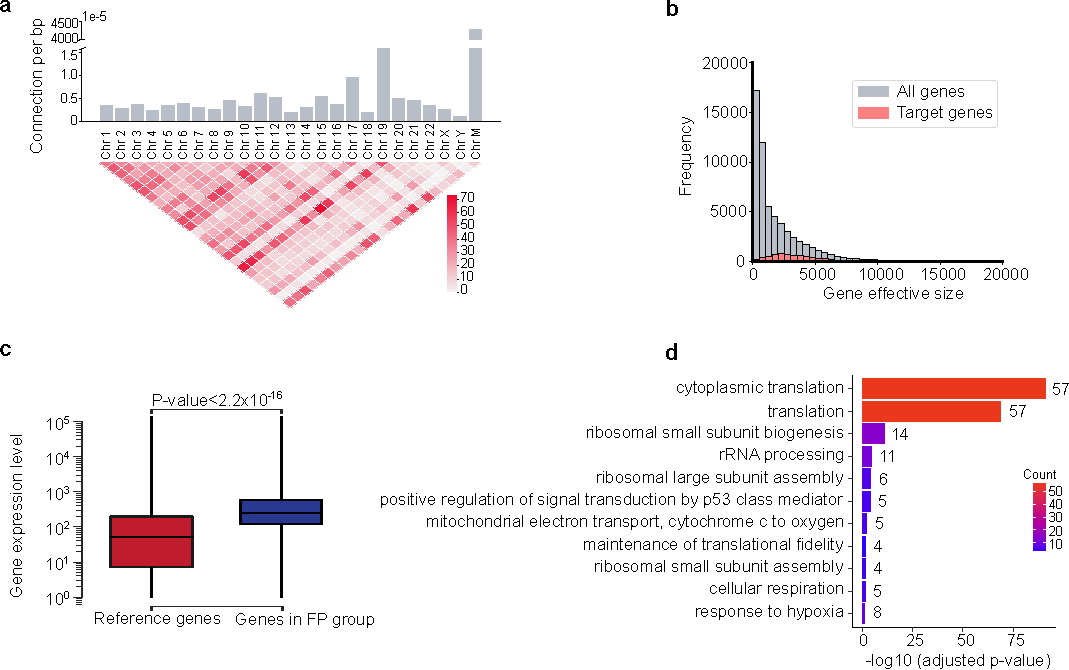
\includegraphics[height=0.73\columnwidth]{finals/sf2}
	\caption{ {\bf Characterization of \gls{fp} chimeric reads Detected by DeepChopper in the VCaP 002 dataset.} 
  (a) Comparison of gene expression levels between reference genes and \gls{fp} genes in the VCaP 002 dataset. \gls{fp} genes show significantly higher expression levels (\(\textrm{p-value} < 2.2 \times 10^{-16}\)). (b) Distribution of gene effective sizes for all genes and target genes, showing similar lengths between reference and \gls{fp} genes. (c) Chromosomal distribution and connections in \gls{fp} chimeric reads of VCaP 004. Top: Bar plot showing the number of connections per base pair (log scale) for each chromosome. Higher bars indicate more frequent connections. Bottom: Heatmap illustrating the count of connections between chromosomes. Intensity of color corresponds to the number of connections.}
	\label{fig:sf2}
\end{figure}


\begin{figure}[!h]
	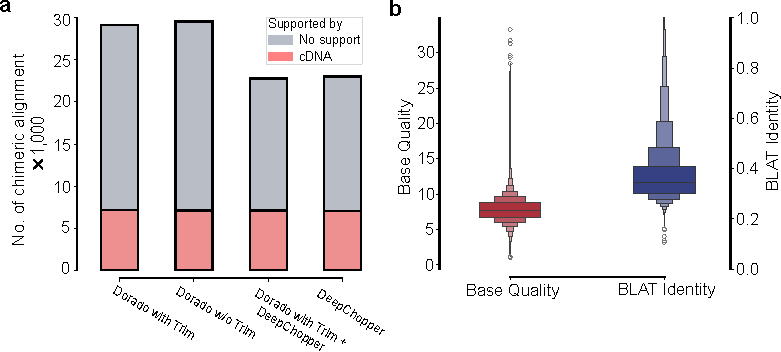
\includegraphics[height=1.2\columnwidth]{finals/sf3}
	\caption{ {\bf Chromosomal connections of fusion events in false positive chimeric reads from VCaP 002 dataset.} Red and blue links indicate intra and inter-chromosomal fusions.}
	\label{fig:sf3}
\end{figure}


\begin{figure}[!h]
	\includegraphics[height=0.87\columnwidth]{finals/sf4}
	\caption{ {\bf  Analysis of \gls{fp} chimeric reads } (a) Distribution of \gls{fp} biological processes enriched among \gls{fp} group genes in HCT116. (b) Distribution of \gls{fp} biological processes enriched among \gls{fp} group genes in MCF7. (c) Distribution of \gls{fp} biological processes enriched among \gls{fp} group genes in K562. (d) Distribution of \gls{fp} biological processes enriched among \gls{fp} group genes in HepG2. (e) Distribution of \gls{fp} biological processes enriched among \gls{fp} group genes in VCaP. (f) Distribution of \gls{fp} biological processes enriched among \gls{fp} group genes in A549.}
	\label{fig:sf4}
\end{figure}



\newpage

\section{Supplementary information}

\renewcommand{\figurename}{Supplementary Fig.}
\renewcommand{\tablename}{Supplementary Table}


% If your article has accompanying supplementary file/s please state so here.
% Authors reporting data from electrophoretic gels and blots should supply the full unprocessed scans for key as part of their Supplementary information. This may be requested by the editorial team/s if it is missing.
% Please refer to Journal-level guidance for any specific requirements.


\begin{table}
	\centering
	\caption{Hyperparameter ranges used}\label{tab:hyperparameter}
	\begin{tabular}{lc}
		\toprule
		                     & {$\sf DeepChopper$}               \\
		\midrule
		Parameters           & 1.6M                              \\
		Optimizer            & AdamW                             \\
		Optimizer momentum   & $\beta_1$, $\beta_2$ = 0.9, 0.999 \\
		Training epoch       & 60                                \\
		Batch size           & 64                                \\
		Learning rate        & 2e-5 to 1e-3                      \\
		LR scheduler         & ReduceLROnPlateau                 \\
		Weight decay (model) & 0-0.2                             \\
		Sequence lengths     & 32769                             \\
		\midrule
	\end{tabular}
\end{table}

% \section*{Declarations}

% Some journals require declarations to be submitted in a standardised format. Please check the Instructions for Authors of the journal to which you are submitting to see if you need to complete this section. If yes, your manuscript must contain the following sections under the heading `Declarations':
%
%\begin{itemize}
%	\item Funding
%	\item Conflict of interest/Competing interests (check journal-specific guidelines for which heading to use)
%	\item Ethics approval and consent to participate
%	\item Consent for publication
%	\item Data availability
%	\item Materials availability
%	\item Code availability
%	\item Author contribution
%\end{itemize}

%
%\begin{appendices}
%	\printglossary[type=\acronymtype, title=Abbreviations]
%
%	\section{Section title of first appendix}\label{secA1}
%
%	An appendix contains supplementary information that is not an essential part of the text itself but which may be helpful in providing a more comprehensive understanding of the research problem or it is information that is too cumbersome to be included in the body of the paper.
%
%	%%=============================================%%
%	%% For submissions to Nature Portfolio Journals%%
%	%% please use the heading ``Extended Data''.   %%
%	%%=============================================%%
%
%	%%=============================================================%%
%	%% Sample for another appendix section			               %%
%	%%=============================================================%%
%
%	%% \section{Example of another appendix section}\label{secA2}%
%	%% Appendices may be used for helpful, supporting or essential material that would otherwise
%	%% clutter, break up or be distracting to the text. Appendices can consist of sections, figures,
%	%% tables and equations etc.


%\end{appendices}

%%===========================================================================================%%
%% If you are submitting to one of the Nature Portfolio journals, using the eJP submission   %%
%% system, please include the references within the manuscript file itself. You may do this  %%
%% by copying the reference list from your .bbl file, paste it into the main manuscript .tex %%
%% file, and delete the associated \verb+\bibliography+ commands.                            %%
%%===========================================================================================%%


%% if required, the content of .bbl file can be included here once bbl is generated
%%\input sn-article.bbl

\end{document}
